\chapter{Trabalhos relacionados}\label{cap:introducao}

Giovanni \citeonline[p.~117]{mori_analysing_2015} define a improvisação de códigos em relação à Música, Imagens em Movimento, Dança ou Tecelagem. É importante esclarecer que essa definição denota a aplicação desta técnica em qualquer outra área, onde o fluxo criativo é essencial:

\begin{citacao}
\traducao{\emph{Live coding} é uma técnica artística de improvisação. Pode ser empregada em muitos contextos diferentes de performance: dança, música, imagens em movimento e mesmo tecelagem. Eu concentrei minha atenção no lado musical, que parece ser o mais proeminente.}{Live coding is an improvisatory artistic technique. It can be employed in many different performative contexts: dance, music, moving images and even weaving. I have concentrated my attention on the music side, which seems to be the most prominent.}
\end{citacao}

Neste trabalho vamos situar a improvisação de códigos do ponto de vista musical. Descartamos uma discussão específica sobre imagens em movimento para evitar cair em uma digressão infinita, já que este é outro campo proeminente. A discussão sobre tecelagem \ver{sec:tecelagem} conecta uma história da computação com a prática investigada. Os exemplos de dança \ver{sec:danca} ilustram duas situações. O primeiro é a Música Eletrônica para Dançar \footnote{\cfcite{hillegonda_dj_2013}.} \ver{sec:algorave}, e o segundo nega o som como resultado da improvisação de códigos \ver{sec:coreografia}. Por último, a característica musical da improvisações de códigos será explorada do ponto de vista histórico \ver{sec:musica}.

\section{Tecelagem}\label{sec:tecelagem}

Contextualizar a atividade têxtil é uma forma de criar uma imagem mental, de como funciona o processo de computação. Seria possível usar a imagem de um ábaco. Mas essa última imagem não considera potenciais leitores de um programa de pesquisa que inclui investigadores na área de Moda (PPG-ACL UFJF). Não aprofundaremos o assunto de Moda, mas sim buscamos ilustrar um código de computador. Nas palavras de \citeonline{griffths_weave2_2015},

\begin{citacao}
 \traducao{Um dos potenciais da tecelagem que eu fiquei mais interessado é a capacidade de demonstrar fundamentos de \emph{softwares} por fios -- parcialmente tornar a natureza física da computação auto-evidente, mas também como uma maneira de modelar novas formas de aprender e a entender o que são os computadores.}{One of the potentials of weaving I’m most interested in is being able to demonstrate fundamentals of software in threads – partly to make the physical nature of computation self evident, but also as a way of designing new ways of learning and understanding what computers are.}
\end{citacao}

\subsection{Charles Babbage e Joseph-Marie Jacquard}

Os computadores atuais são máquinas desenvolvidas com base no modelo teórico elaborado por Alan Turing (1912-1954). Uma representação simplista considera uma fita abstrata de tamanho variável (o quanto for necessário), dividida em células, cada uma com um alfabeto finito. Cada alfabeto possui uma quantidade de símbolos de representação finita. Um cabeçote leitor desta fita lê as instruções escritas em cada célula, e depois passa para a próxima célula. Um registrador de estados desta fita, memoriza qual foi a última operação realizada na última célula executada. Uma tabela de ações indicará novas instruções, que serão escritas nesta fita.

 Um modelo anterior ao de Turing foi elaborado por Charles Babbage (1791 -- 1871), \emph{a máquina analítica},  entre 1834 e 1836, revisado em 1837. Sua construção ocorreu após um colapso na construção de sua \emph{máquina diferencial}. O projeto não vingou, mas a partir de 1838, Babbage se envolveu com a exploração intelectual dos conceitos elaborados, para otimizar o projeto e reduzir seu custo de construção. Uma sequência de seminários em Turin (1840) resultou em uma publicação sobre a máquina analítica, em francês, escrita por um cientista italiano (L.F. Menebrea). A Condessa de Lovelace (Ada Augusta Byron King), traduziu, sob supervisão de Babbage, esta publicação para o inglês. Historicamente, os primeiros programas de computador (para serem executados na máquina analítica) foram escritos ambos por Ada e Babbage. O primeiro programa escrito era dedicado ao cálculo de uma sequência numérica conhecida como \emph{Números de Bernoulli} \footnote{Allan G. Broomley, \emph{Charles Babbage’s Analytical Engine, 1838}. Disponível em \url{http://athena.union.edu/~hemmendd/Courses/cs80/an-engine.pdf}}. Apenas uma parte da máquina foi construída antes da morte de Babbage\disponivelem{http://www.sciencemuseum.org.uk/objects/computing_and_data_processing/1878-3.aspx}.

Segundo \citeonline[p.14--21]{McLean2011}, o mecanismo do projeto de Babbage é inspirado na máquina de tear de Joseph-Marie Jacquard (1752 -- 1834). A principal contribuição da invenção, para a computação, foi um sistema que consiste em um cabeçote leitor de cartões perfurados. Na máquina de tear de Jacquard, a organização dos furos indicam, até hoje, uma rotina têxtil \ver{fig:jacquard}. Já no computador mecânico de Babbage, o cartão perfurado indicava estados binários que conduzem ao cálculo numérico:

\begin{citacao}
\traducao{A indústria têxtil vislumbrou a primeira máquina programável de ampla utilização: a cabeça de tear Jacquard, uma tecnologia ainda usada. Longas tiras de cartão são alimentados na cabeça de tear Jacquard, que lê padrões perfurados no cartão para guiar a intrincada padronização de tecidos. O cabeçote Jacquard não computa, mas foi admirado por Charles Babbage, inspirando o trabalho na sua máquina analítica mecânica, a primeira concepção de um computador universal programável. Embora Babbage não tenha obtido sucesso em construir a máquina analítica, seu projeto inclui um mecanismo de entrada de cartão similar ao cabeçote Jacquard, mas com  padrões perfurados descrevendo cálculos abstratos ao invés de fios têxteis.}{
The textile industry saw the first programmable machine to reach wide use: the head of the Jacquard loom, a technology still used today. Long strips of card are fed into the Jacquard head, which reads patterns punched into the card to guide intricate patterning of weaves. The Jacquard head does not itself compute, but was much admired by Charles Babbage, inspiring work on his mechanical analytical engine (Essinger, 2004), the first conception of a programmable universal computer. Although Babbage did not succeed in building the analytical engine, his design includes a similar card input mechanism to the Jacquard head, but with punched patterns describing abstract calculations rather than textile weaves.
}
\end{citacao}

\begin{figure}[!h]
  \centering
  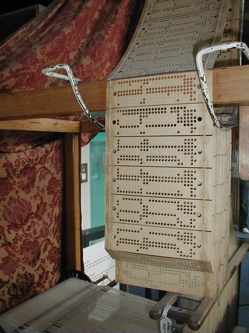
\includegraphics[scale=0.82]{imagens/Jacquard.jpg}
  \caption{Cartões perfurados da máquina de tear Jacquard. \textbf{Fonte}: wikimedia.org }
  \label{fig:jacquard}
\end{figure} 

\subsection{Weavecoding}\label{sec:weavecoding}

Se até hoje o mesmo sistema de Jacquard é utilizado, e considerado que a indústria têxtil possui suas aplicações computacionais, como improvisadores de códigos realizam uma bricolagem de improvisação audiovisual, computação e atividade têxtil? Exemplificamos o caso com um grupo que criou o conceito \emph{weavecoding}. Para definí-lo, ilustramos uma investigação informal (um encontro de acadêmicos e não-acadêmicos no Foam Kernow\disponivelem{http://fo.am/kernow/}).

O grupo \emph{Weaving codes}\disponivelem{http://kairotic.org/about/} foi formado para  investigar \traducao{padrões a partir das perspectivas de tecelagem e música, e através do desenvolvimento de uma linguagem de computador e código para descrever a construção de tecidos}{We pursue these questions in the Weaving Codes- Coding Weaves project, by investigating patterns from the perspectives of weaving and music, and by developing a computer language and code for describing the construction of weaves}. É formado por membros da Universidades de Leeds, Nottingham Trent, Cambridge, Aberdeen, Copenhague; um museu (\emph{Albert Museum}), uma rede de laboratórios transdisciplinares (FoAM Kernow ); o Centro Dinamarquês para Pesquisa Têxtil, e Escola Robert Schumman de Música e Mídia de  Düsseldorf. 

Uma pequena digressão: dois membros deste grupo, Alex McLean e Dave Griffths, são praticantes e organizadores de improvisações de código como artistas-programadores. A principal contribuição dos autores provavelmente foi a divulgação de uma heurística para uma improvisação com computadores, \emph{Lubeck04}, mais conhecido como \traducao{Mostre-nos suas telas}{Show Us Your Screens}, dentro de um manifesto publicado como \traducao{Programação de Algoritmo Ao vivo e Organização Temporária para sua Promoção}{Live Algorithm Programming and Temporary Organization for its Promotion} \cite{ward_live_2004}. Este tema será discutido adiante \ver{sec:showusyourscreens}.

Do manifesto à codificação têxtil, \citeonline{griffths_weave2_2015} apresenta um interessante exemplo. A partir de quatro tarefas fundamentais (rotinas), descritas no Exemplo \autoref{ex:weaving}, é possível elaborar um padrão como o apresentado na \autoref{fig:weaving}. A primeira rotina é \emph{repeat}, uma repetição de ações por contagem $[$\emph{loop}$]$; a segunda é \emph{twist}, ou dar a volta em determinados pontos; a terceira,  \emph{weave-forward}, tecer à frente do ponto; e a quarta, \emph{weave-back}, tecer atrás do ponto . Do lado direito da imagem (ver p.~\pageref{fig:weaving}), é simbolizado o ``código criptografado de tecido'', ou as operações fundamentais para um determinado padrão têxtil. Do lado esquerdo, seu resultado-padrão, uma textura de losangos e zigue-zagues.  

\begin{example}{Um código-fonte que gera um tecido semelhante à \autoref{fig:weaving}.}
\label{ex:weaving}
\begin{minted}[fontsize=\footnotesize]{cl}
(twist 3 4 5 14 15 16)
(weave-forward 3)
(twist 4 15)
(weave-forward 1)
(twist 4 8 11 15)

(repeat 2
 (weave-back 4)
 (twist 8 11)
 (weave-forward 2)
 (twist 9 10)
 (weave-forward 2)
 (twist 9 10)
 (weave-back 2)
 (twist 9 10)
 (weave-back 2)
 (twist 8 11)
 (weave-forward 4))
\end{minted}
\end{example}

\begin{figure}[!h]
    \centering
    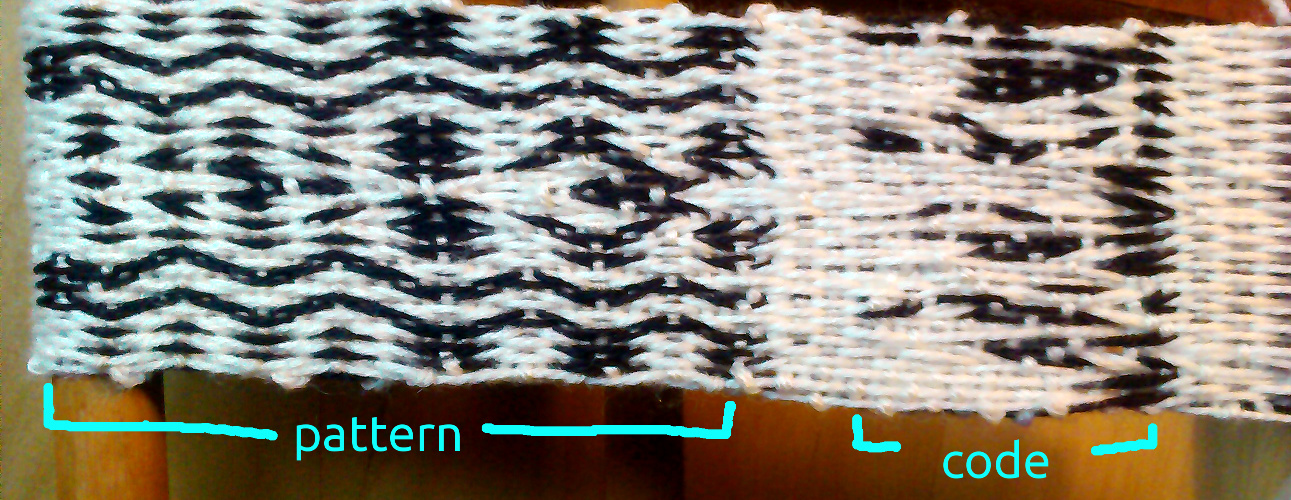
\includegraphics[scale=0.31]{imagens/weaving.jpg}
    \caption{Tecido resultante da prática \emph{Weaving code}. \textbf{Fonte}: \citeonline{griffths_weave2_2015}.}
  \label{fig:weaving}
\end{figure}

Esta experiência de \emph{weavecoding} pode ser aplicada em uma performance \ver{fig:weavecoding}. Griffths ilustra uma performance arquetípica da improvisação de códigos: programadores escrevendo enquanto os resultados são projetados em superfícies planas. Como veremos, é interessante que o que está sendo escrito também seja projetado \cite[p.~129]{McLean2011}, o que não é o caso desta imagem. A tecelagem é programada por meio de um dispositivo tangível \ver{fig:weavecoding2}, uma matriz de botões acopláveis, desenvolvida por Ellen Harlizius-Klück (investigadora da história da matemática, filosofia e tecelagem da Grécia Antiga na Universidade de Copenhague\disponivelem{http://www.saumweberei.de/}) e Alex McLean \ver{fig:weavecoding2}. Imagens em movimento foram projetadas como capturas das atividades têxteis e processadas por Griffths. 

\begin{figure}[!h]
  \centering
  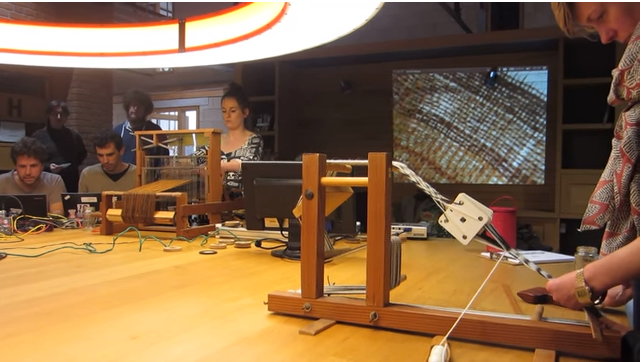
\includegraphics[scale=0.71]{imagens/weaving.png}
  \caption{Performance no Foam Kernow. \textbf{Fonte}: \citeonline{griffths_weave_2015}.}
  \label{fig:weavecoding}
\end{figure}

\begin{figure}[h]
  \centering
  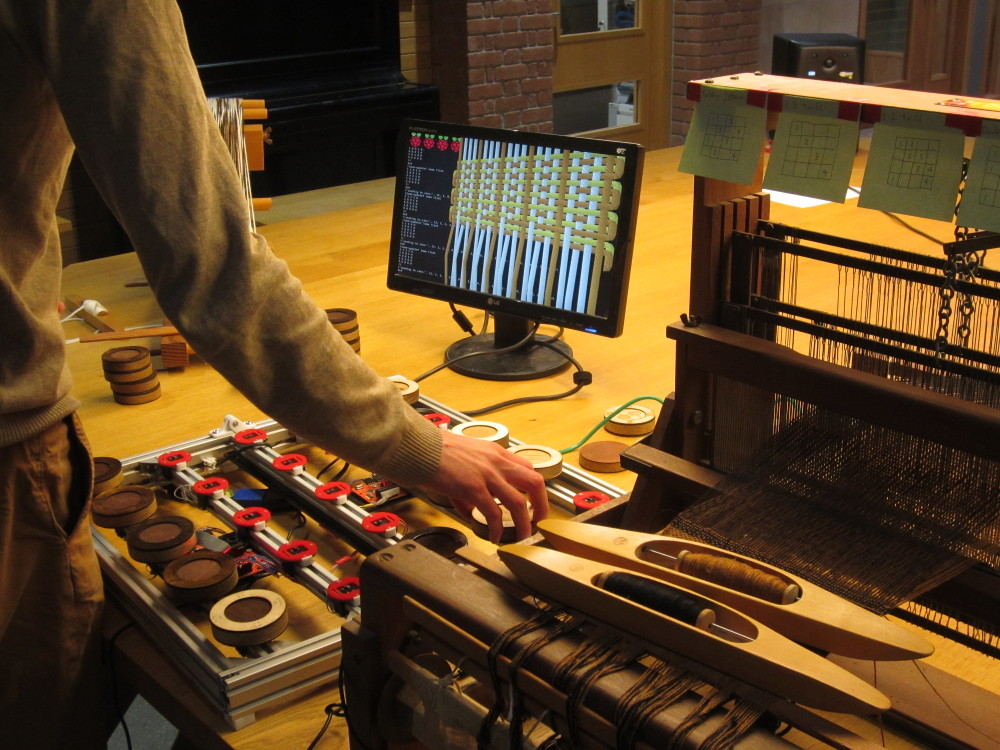
\includegraphics[scale=0.85]{imagens/weavecoding.jpg}
  \caption{ Alex McLean manipulando uma Matriz de botões para tecelagem, conectado a um Raspberry Pi. \textbf{Fonte}: \citeonline{griffths_weave_2015}.}
  \label{fig:weavecoding2}
\end{figure}

\begin{citacao}

\traducao{
Uma das idéias originais era combinar tecelagem e codificação em um cenário de atuação, ambos para fornecer uma forma de tornar a codificação ao vivo mais inclusiva com a tecelagem, e ao mesmo tempo esclarecer os processos de pensamentos digitais envolvolvidos na tecelagem (\ldots) Nossa audiência consistiu de pesquisadores de artesanato, biólogos antropológicos, arquitetos, designers de jogos e tecnólogos -- foi mais do que antecipamos! Alex e eu disponibilizamos alguns códigos de música do \emph{slub} para tecer, e minha parte favorita foi projetar a tecelagem ao vivo.
}{
One of the original ideas we had was to combine weaving and coding in a performance setting, to both provide a way to make livecoding more inclusive with weaving, and at the same time to highlight the digital thought processes involved in weaving. (\ldots) Our audience consisted of craft researchers, anthropological biologists, architects, game designers and technologists -- – so it all went on quite a lot longer than we anticipated! Alex and I provided some slub livecoded music to weave by, and my favourite part was the live weaving projection.
}
\end{citacao}

\todo[color=lightred]{\tiny está faltando ligação entre este parágrafo e o anterior}

Esta descrição de Griffths possui uma domentação audiovisual \disponivelem{https://www.youtube.com/watch?v=XrnIVUp9QgM}. É interessante notar que a menção ao grupo \emph{Slub} auxilia a discussão musical. Por hora apenas mencionamos sua inserção no cenário da Música Eletrônica de Dança\footnote{\cfcite{hillegonda_dj_2013}}. Subgêneros como \emph{rave}, \emph{gabba} e \emph{rotterdam}, são algumas das principais categorizações musicais\footnote{\cfcite{janotti_jr._a_2003,sa_musica_2006,sa_se_2009}} aplicadas à improvisação de códigos \ver{sec:algorave}.


\section{Dança}\label{sec:danca}

A Dança é ilustrada de duas maneiras. A primeira é dança como fim de uma improvisação musical. O segundo caso foge do escopo sonoro; uma coreógrafa codifica apenas a orientação espacial de uma bailarina, resultando em uma sensação de quietude sonora. É uma posição que diverge da maioria dos trabalhos apresentados, mas é pouco discutido no âmbito musical.

\subsection{Algorave}\label{sec:algorave}

A compositora colombiana Alexandra Cárdenas, em entrevista com \citeonline{chesire_algorave_2013}, cita Nick Collins e Alex McLean como os criadores do termo \emph{algorave}. Surgiu durante uma \emph{gig} (um termo utilizado no início do \emph{jazz} para caracterizar um trabalho temporário). Após sintonizarem em uma estação de rádio, decidiram codificar uma música semelhante:

\begin{citacao}
\traducao{
Algorave 'comecou como uma piada', de acordo com Alex McLean, um pesquisador de música computacional e um dos três de uma banda chamada \emph{Slub}, que têm improvisado códigos por 13 anos. Ele veio com um termo enquanto conduzia uma \emph{gig} em Nottingham com seu amigo Nick Collins (que tocava ``datapop'' sob o nome Sick Lincoln) no final de 2011. 'Nós sintonizamos em uma estação pirata tocando \emph{happy hardcore}, e nós pensamos que seria bom programar alguma música \emph{rave}.' Deste então, McLean organizou oito \emph{algoraves} informais no mundo.
}
{
Algorave "started as a joke", according to Alex McLean, a computer-music researcher and one-third of a band called Slub that's been live coding for 13 years. He came up with the term while driving to a gig in Nottingham with his friend Nick Collins (who plays "datapop" under the name Sick Lincoln) in late 2011. "We tuned into a pirate station playing happy hardcore, and we thought it would be good to program some rave music." Since then, McLean has organised eight informal algoraves around the world. 
}
\end{citacao}

Em seu artigo ``Algorave: Live Performance of Algorithmic Electronic Dance Music'', \citeonline[p.~356]{collins_algorave_2014} sustentam que as estruturas das práticas do \emph{algorave} são anteriores à improvisação de códigos, e já era utilizado na Música Eletrônica para Dançar. O que mantêm a relação entre os dois é a prática de projeção do código \ver{sec:laptoptoplap}.

\begin{citacao}
\traducao{
\emph{Algorave} não é sustentado exclusivamente por \emph{live coders}, mas estes têm mantido uma forte presença em todos os eventos até agora. É assim talvez porque a tradição do \emph{live coding} de projetar telas motiva todo o esforço; onde algoritmos não estão visíveis por períodos de tempo durante uma \emph{algorave}, se corre o risco das coisas parecerem muito como um evento de música eletrônica padrão.
}
{Algorave is not exclusively a preserve of live coders, but they have maintained a strong presence at every event thus far. This is perhaps because the live coding tradition of projecting screens help motivates the whole endeavour; where algorithms are not made visible for periods during an algorave, we run the risk of things feeling much like a standard electronic music event.}

\end{citacao}

Focando no aspecto histórico, \citeauthoronline{collins_algorave_2014} descrevem uma sequência de eventos (desenvolvimentos de \emph{softwares} e apresentações). Em 1992, Charles Ames disponibiliza o \emph{Cybernetic Composer}, \traducao{um \emph{software} com um sistema baseado em Inteligência Artificial que compõe musica em uma variedade de estilos populares.}{an AI based software system that composes music in a variety of popular styles. Disponível em \url{http://www.kurzweilai.net/charles-ames}}. Em 1994, o duo \emph{Koan}, formado pelos DJs Daniel Roeth e William Grey, realizam adaptações para entretenimento com base no \emph{ambient music} de Brian \citeonline{eno_music_1978}. \emph{Aphex Twin} (Richard David James) cria em 1997 o termo \emph{live club algorithm}. Em 1999, o protocolo para edição audiovisual ao vivo \emph{bbcut} \cite{collins_bbcut_2003} é incluído nos \emph{opcodes} do \emph{CSound}\footnote{Disponível em \url{https://csound.github.io/}.}, e do \emph{Supercollider}. Em 2000 o então duo \emph{Slub}, realizam performances, autodenominadas \emph{generative techno}, com abordagem \emph{gabba}. Em 2001 é identificado a utilização de redes neurais para composição de padrões semelhantes ao \emph{drum'n'bass}. Em 2004 é fundado o TOPLAP em uma casa noturna de Hamburgo.

Ilustramos três casos recentes, onde a improvisação de códigos é uma técnica utilizada. Junto com a improvisação de códigos, são utilizados um instrumento eletrônico, voz, e um instrumento elétrico. O inglês Canute, o mexicano Mico Rex e a colombiana residente na Alemanha, Alexandra Cárdenas.

\begin{figure}[!h]
  \centering
  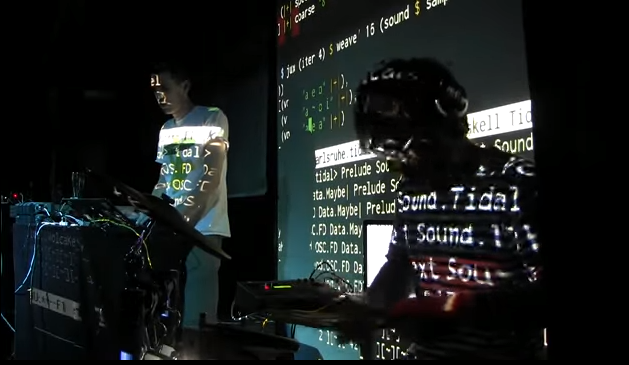
\includegraphics[scale=0.71]{imagens/canute.png}
  \caption{Performance do duo Canute (Karlesruhe, 2015) \textbf{Fonte}: \url{https://www.youtube.com/watch?v=uAq4BAbvRS4}.}
  \label{fig:canute}
\end{figure}

O registro audiovisual do duo Canute, Matthew Yee-King e Alex McLean, reforça improvisos de códigos arquetípicos \ver{fig:canute}. Aqui a projeção segue à risca duas recomendações, ``Mostre-nos suas telas''\label{sec:showusyourscreens} e ``Obscurantismo é perigoso''\ver{sec:obscurantismo}. Os instrumentos utilizados são um \emph{laptop} e uma bateria eletrônica.  McLean improvisa códigos, escritos no ambiente de programação \emph{Tidal} \ver{sec:tidal}. 


O registro audiovisual cita termos como \emph{club} e \emph{chordpunch}. Estes descrevem gêneros musicais para o código improvisado. É importante lembrar que McLean também utiliza outras categorizações musicais em outras performances. É curioso notar que em alguns momentos do vídeo, certas modificações nos códigos causam uma perturbação brusca em sistema de ritmos (percebido pelo fluxo musical); em alguns momentos Yee-King mantêm o fluxo, mas em outros o instante musical codificado leva um curto período de tempo para ser sincronizado. Sugerimos que este não é  \emph{a priori} um erro do instrumentista, mas sim de questões de performance que serão mencionados na \autoref{sec:showusyourscreens}.

Griffiths registra uma \emph{rave} na embarcação  MS Stubnitz, em Canary Wharf, Londres, em 2013. Cárdenas e Ernesto Romero/Jorge Ramírez (Mico Rex, \autoref{fig:micorex}) tocam neste evento. Encontramos um registro audiovisual de curta duração da apresentação do duo Mico Rex\disponivelem{https://vimeo.com/65309754}, mas não de Cárdenas. Exemplos sonoros específicos estão disponíveis nas redes sociais \emph{SoundCloud} e \emph{Vimeo} \footnote{\url{https://soundcloud.com/tiemposdelruido} e \url{https://soundcloud.com/micorex/}.}.

\begin{figure}[!h]
  \centering
  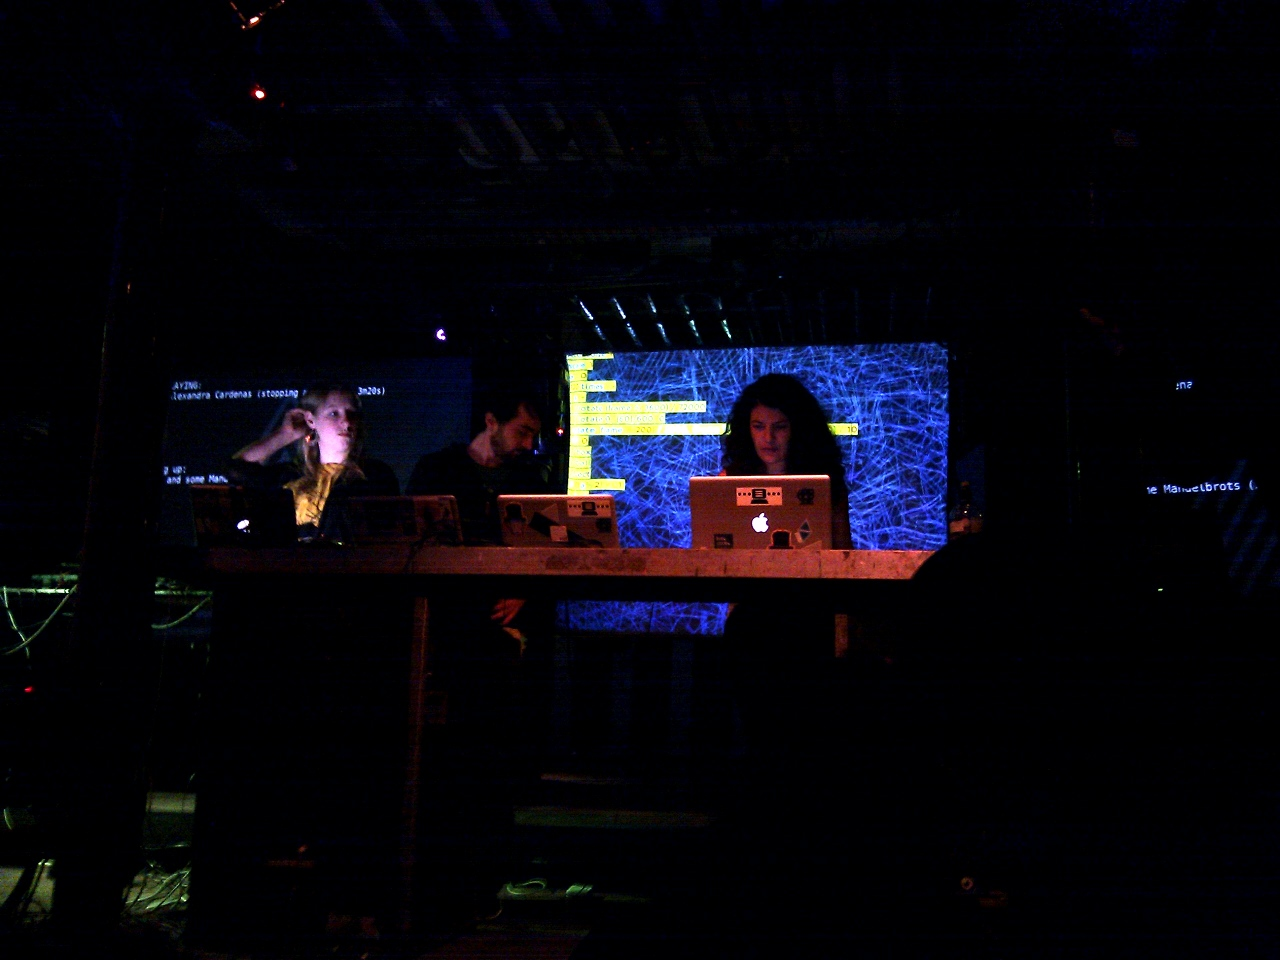
\includegraphics[scale=0.31]{imagens/cardenas.jpg}
  \caption{Performance do duo Mico Rex (Londres, 2013) \textbf{Fonte}: \url{http://www.pawfal.org/dave/blog/tag/algorave/}.}
  \label{fig:cardenas}
\end{figure}

Notas descritivas especificam instrimentos e linguagens de programação. MicoRex utiliza voz e \emph{programação} ao vivo com o ambiente de programação SuperCollider. Realiza performances de \emph{electro-pop}, \emph{8bits/glitch}, \emph{electro}, \emph{punk} e \emph{breakz}\disponivelem{http://algorave.com/micorex/}. Cárdenas realiza suas performances com guitarra e programação ao vivo com o SuperCollider. É interessante lembrar que Cárdenas possui uma formação em Composição e Violão clássico na Universidade de Los Andes\disponivelem{http://cargocollective.com/tiemposdelruido/Alexandra-Cardenas} e que além de recorrerer ao \emph{techno} e \emph{dubstep}, se apropria do \emph{noise} através de distorções, e composição mista de retroalimentação de sinais em instrumentos expandidos (como a utilização de objetos diversos na guitarra em conjunto com Processamento Digital de Sinais).

\begin{figure}[!h]
  \centering
  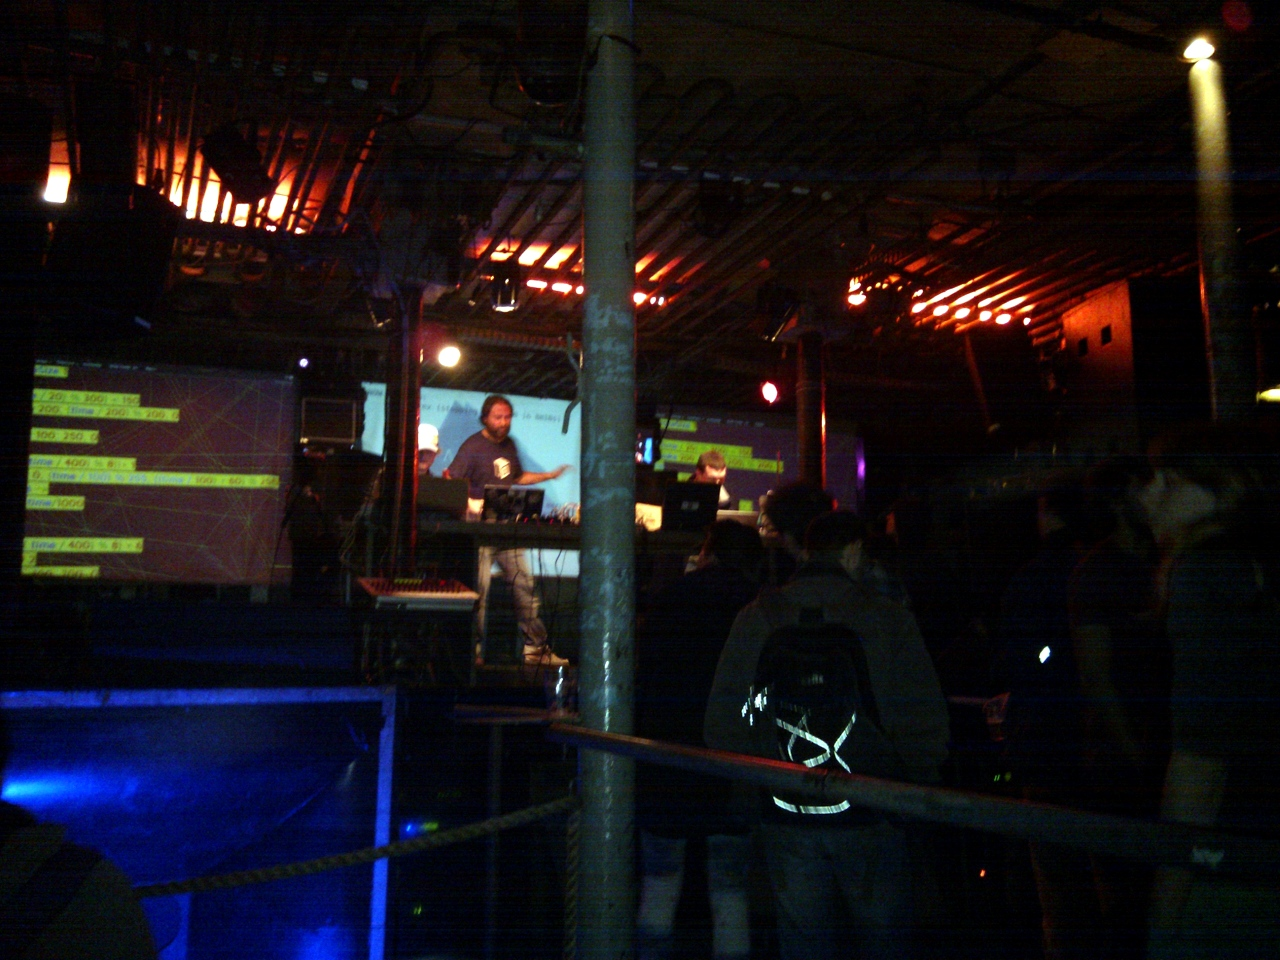
\includegraphics[scale=0.31]{imagens/algorave.jpg}
  \caption{Performance do duo Mico Rex (Londres, 2013) \textbf{Fonte}: \url{http://www.pawfal.org/dave/blog/tag/algorave/}.}
  \label{fig:micorex}
\end{figure}

O SuperCollider\disponivelem{https://supercollider.github.io/} é um ambiente de programação desenvolvido por James McCartney. Realiza síntese sonora em \emph{tempo real}\ver{sec:jit} e permite a programação de rotinas musicais\ver{fig:sc}. O exemplo \autoref{ex:artificial} um código de Frederick Olofson que ilustra uma codificação de uma sonoridade de \emph{games}, recorrente no \emph{algorave}.  Um sintetizador recria o timbre do videogame \emph{Atari2600} (laçado no EUA em 1977); mais especificamente é um simulador do \emph{chip} TIA (\emph{Television Interface Adapter}), responsável pela geração de gráficos e imagens no videogame\disponivelem{https://www.atariage.com/2600/archives/schematics_tia/index.html}. O exemplo é relativamente simples; a frequência portadora do sintetizador segue padrões de movimentos brownianos diferentes que variam entre 28 e 31 $Hz$, alternados com 23 e 26 $Hz$. Enquanto isso a frequência moduladora segue um padrão repetitivo que alterna 10 e 16 $Hz$ com 11 e 16 $Hz$.

\begin{figure}[!h]
  \centering
  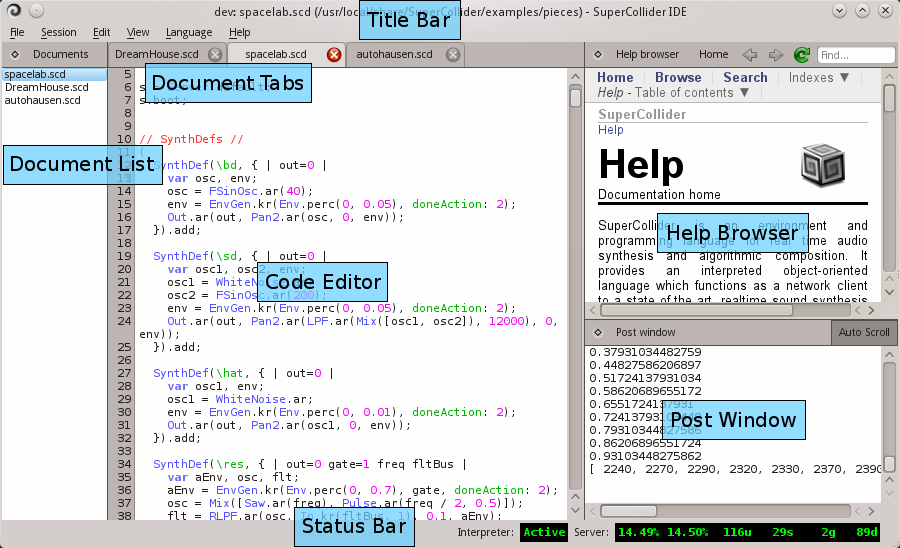
\includegraphics[scale=0.31]{imagens/sc_ide_overview.png}
  \caption{Ambiente de programação e composição \emph{SuperCollider}. \textbf{Fonte}: \url{https://supercollider.github.io/}.}
  \label{fig:sc}
\end{figure}

\begin{example}{Definição de uma unidade sonora e sua execução}
\textbf{Fonte}: \url{http://supercollider.sourceforge.net/audiocode-examples/}

\begin{lstlisting}[style=SuperCollider-IDE]
// Simple synth definition using the Atari2600 UGen:
(
SynthDef(\atari2600, {|out= 0, gate= 1, tone0= 5,
tone1= 8, freq0= 10, freq1= 20, amp= 1, pan= 0|
  var e, z;
  e= EnvGen.kr(Env.asr(0.01, amp, 0.05), gate, doneAction:2);
  z= Atari2600.ar(tone0, tone1, freq0, freq1, 15, 15);
  Out.ar(out, Pan2.ar(z*e, pan));
}).store
)

// And a pattern to play it:
(
Pbind(
  \instrument, \atari2600,
  \dur, Pseq([0.25, 0.25, 0.25, 0.45], inf),
  \amp, 0.8,
  \tone0, Pseq([Pseq([2, 5], 32), Pseq([3, 5], 32)], inf),
  \tone1, 14,
  \freq0, Pseq([Pbrown(28, 31, 1, 32), Pbrown(23, 26, 3, 32)], inf),
  \freq1, Pseq([Pn(10, 16), Pn(11, 16)], inf)
).play
)
\end{lstlisting}
\end{example}\label{ex:artificial}


\subsection{Coreografia}\label{sec:coreografia}

A segunda situação de ``dança'' é ilustrada na \autoref{fig:iclcdanca}, com uma performance coreografada por  Kate Sicchio (2015). Envolve ambientes de apresentação formal (teatros, auditórios), como na performance \emph{HTB2.0} de Kate Sicchio\disponivelem{https://www.youtube.com/watch?v=iOAffWTBVE0}. A coreografia segue uma partitura, que é codificada durante a performance. Uma bailarina improvisa movimentos conforme o que está indicado na partitura. No entanto sua conexão com a partitura não é visual ou sonora, e sim tátil:

\begin{citacao}
\traducao{Esta peça é uma exploração de eletrônica codificada ao vivo e movimentos improvisados. Uma dançarina veste uma peça de atuadores táteis. Estes atuadores são programados em tempo-real via OSC\footnote{N.A.: ``\emph{Open Sound Control} é um protocolo de comunicação entre computadores, sintetizadores sonorosm e outros dispositivos multimídia que são otimizados para as modernas tecnologias de rede''. Disponível em \url{http://opensoundcontrol.org/introduction-osc}} para 'zunir' sobre os lados direito e esquerdo da dançarina para indicar qual lado do corpo a dançarina deve mover. A partitura é codificada ao vivo pela coreógrafa enquanto a dançarina responde por uma retroalimentação háptica. Esta peça explora o \emph{live coding} de corpos, e movimento como saída, ao invés de saídas sonoras ou visuais como encontrado em muitas execuções de \emph{live coding}
}{
This dance piece is an exploration of live coded electronics and improvisational movement. A dancer wears a custom garment of haptic actuators. These actuators are programmed real-time via OSC to 'buzz' on the right and left sides of the dancer to indicate which side of the body the dancer will move. The score is being live coded by choreographer while the dancer is responding to the haptic feedback. This piece explores live coding of bodies and movement as output rather than a sonic or visual output as found in many live coding performances.
}
\end{citacao}

\begin{figure}[!h]
  \centering
  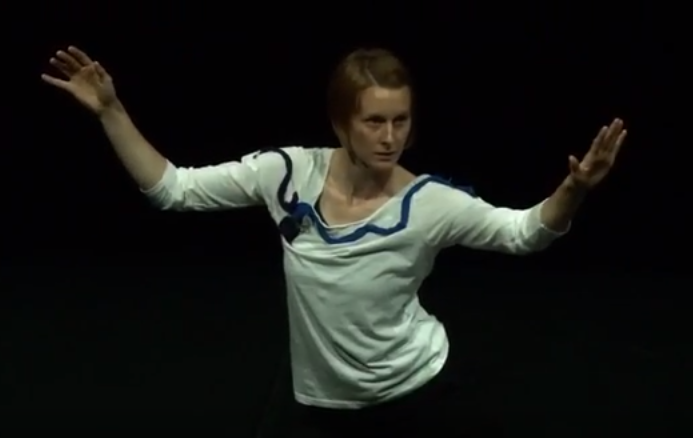
\includegraphics[scale=0.6]{imagens/iclcdanca.png}
  \caption{Dançarina (anônima) controlada por Kate Sicchio através de uma codificação improvisada. \textbf{Fonte}: \url{https://www.youtube.com/watch?v=uAq4BAbvRS4}.}
  \label{fig:algorave}
\end{figure}

É interessante notar uma sensação de quietude sonora na performance. Como aponta a própria coreógrafa, a maioria das performances de improviso de códigos segue o seguinte procedimento: o código é criado, e um som, uma nota, uma imagem ou um vídeo são gerados, combinados, transformados. Mesmo em algumas performances de daça pesquisadas, a dança aparecia como um ornamentoou um suporte para a projeção audiovisual. A criatividade deste trabalho toca um conceito técnico fundamental da computação: qual é o \emph{dispositivo de entrada e de saída} praticado nas improvisações de códigos? Sicchio responde o corpo já é um dispositivo de entrada e saída de interações sociais e pode ser controlado por outro humano através de comandos de rede.  


\section{Música}\label{sec:musica}

A situação ``musical'' será exemplificada de duas maneiras. A primeira é a performance de concerto. A segunda será exemplificada como performances telepresenciais e virtuais.

Um exemplo recente do primeiro caso é o improviso \emph{screenBashing} de Magno Caliman (ver \autoref{fig:screenbashing}), realizado durante o XIII ENCUN\footnote{Encontro Nacional de Compositores Universitários em Campinas-SP no ano de 2015.}. Será útil para ilustração de uma \traducao{(\ldots) performance de \emph{livecoding} arquetípica $[$que$]$envolve programadores escrevendo códigos no palco, com suas telas projetadas para a audiência}{The archetypal live coding performance involves programmers writing code on stage, with their screens projected for an audience}\cite[p.~1]{mclean_tidal_2010}

O executante senta-se ao computador como um pianista, com uma penumbra usual dos sistemas de iluminação das casas de concerto. Uma tela de projeção expõe o estado atual de seu \emph{laptop}: um editor de texto é aberto e o executante começa a programar em linguagem C, uma pequena iteração (\emph{for loop}) que repete caracteres diversos, que serão improvisados ao longo do concerto. Assim que termina de escrever um pequeno programa, o executante abre um console (ou terminal nos sistemas operacionais Unix) e solicita para o sistema operacional (no caso um Mac OsX) compilar o programa. A compilação é um processo no qual a representação textual humana é convertida em uma linguagem apropriada para o computador. Este processo não demora, e o programa é executado. O resultado é uma sequência de caracteres de texto como texturas visuais, semi-transparentes. E tudo isso com uma sensação de quietude sonora.  O executante então abre códigos preparados no ambiente de programação  \emph{SuperCollider}\disponivelem{https://supercollider.github.io} para síntese de texturas sonoras ruidosas. Um novo programa visual, na linguagem C, é improvisado e sobreposto à imagem anterior. Um novo som de textura ruidosa é adicionado. Este processo é repetido até o fim da peça. A acumulação dos sons às imagens cria um contínuo sonoro sincrético, que exige cada vez mais e mais do processamento do computador. A improvisação finaliza com um congelamento do sistema operacional, em razão deste acúmulo de memória.

\begin{figure}[!h]
  \centering
  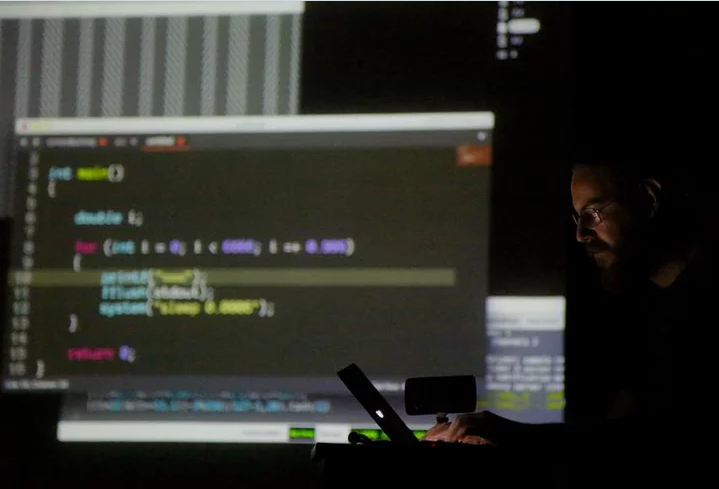
\includegraphics[scale=0.5]{imagens/screenbashing.png}
  \caption{Performance de \emph{screenBashing}. \textbf{Fonte}: \url{https://vimeo.com/148626379}.}
  \label{fig:screenbashing}
\end{figure}

\subsection{Telepresença e espaços virtuais}

Até agora comentamos performances presenciais, mas também existem os exemplos virtuais. Podem usar imagens em movimento no caso de um \emph{live coding} preocupado com texturas visuais. Mas no caso de uma performance ``musical'', esta característica pode ser suprimida. 

Uma performance virtual de \emph{live coding} é aquela em que dois ou mais executantes, em locais diferentes mas conectados pela \emph{internet}, compartilham do mesmo código. Por compartilharem do mesmo código podem também compartilhar do mesmo som. Um detalhe pode dividir esta performance entre telepresenciais e assíncronas. Enquanto a performance telepresencial necessita compartilhar o som digitalizado, na performance assíncrona esta característica é delegada individualmente para cada executante.  

\citeonline[p.~152--153]{junior_supercopair_2015} descrevem uma performance telepresencial em 2014, por Ben Swift, Henry Gardner e Andrew Sorensen, realizada \traducao{entre dois intérpretes-programadores localizados na Alemanha e Estados Unidos usando um servidor SSH localizado na Australia}{between two live coders located in Germany and United States using an SSH server located in Australia.}.  \citeauthoronline{junior_supercopair_2015} ainda descrevem um esforço conjunto de performance remota entre  O autor ainda descreve um esforço Por outro lado, execuções remotas assíncronas (isto é, entre duas ou mais pessoas, em tempos diferentes) são realizadas em \emph{softwares} como \emph{Gibber} \cite{roberts_gibber:_2012}\disponivelem{http://gibber.mat.ucsb.edu/} e \emph{Wavepot}\disponivelem{http://www.wavepot.com}.    

\subsection{Proto-história}\label{sec:protohistoria}

O \emph{Universo de Conceitos} do \emph{live coding} contêm numerosos exemplos. Expomos alguns \emph{Espaços Conceituais} através de exemplos recentes. Se existem outras abordagens, musicalmente e visualmente diversas, a improvisação é o tema articulador. Seria possível dizer que cada uma cria seu próprio \emph{Sistema Criativo} \citeonline{mclean_music_2006}. Métodos de análise que expliquem cada uma dessas improvisações, como \emph{Modelos de Improvisação} ainda é um campo em exploração, através de investigações de \emph{Inteligência Artificial}. Neste sentido, este capítulo busca construir espaços conceituais, e especialmente aqueles citados como ``proto-históricos'', isto é, cujas características são semelhantes (ou remeteram algo para o autor deste documento) ao conjunto de regras práticas publicadas por \citeauthoronline{ward_live_2004}.

Na \autoref{sec:grossi}, \citeonline{mori_pietro_2015}  descreve um caso prematuro de \emph{live coding} na Itália, com o compositor Pietro Grossi (1917-2002). Divergente em algumas das propostas de Max Mathews, sacrificou a questão timbrística para trabalhar na questão performática.

Descrevemos, na seção \autoref{sec:baiasaofranscisco}, as atividades dos grupos \emph{The Hub} e \emph{The League of Automatic Composers} como fundamentais para o entendimento histórico do \emph{live coding}.

Sugerimos na \autoref{sec:jit} apontar a tecnologia JIT \cite{aycock_brief_2003} como um sujeito sócio-técnico fundamental para que o \emph{live coding} fosse possível.

Um recorte do documento-manifesto ``\emph{Live Algorithm Programming and Temporary Organization for its Promotion}'', de \citeauthoronline{mclean_patterns_2009}, será feita na \autoref{sec:laptoptoplap} para discutir identidade cultural da organização TOPLAP. 

Na \autoref{sec:showusyourscreens}, ``Show us your screens'', é revisto como o manifesto que define as regras práticas do \emph{live coding}.

Na \autoref{sec:obscurantismo}, revemos a ideologia de projeção de telas.

%\subsection{GRASS}

\subsection{Pietro Grossi}\label{sec:grossi}

Embora pouco conhecido no contexto geral da música européia, o compositor Pietro Grossi foi  um dos pioneiros da \emph{Computer Music} Italiana. O pensamento musical que rege seus programas de computador sacrifica questões timbrísticas para concentrar na performance. O primeiro \emph{software} desenvolvido foi o DCMP (\emph{Digital Computer Music Program}) e, segundo \citeonline[p.~126]{mori_pietro_2015}, ao usar este programa,

\begin{citacao}
(\ldots) o intéprete era capaz de produzir e reproduzir música em tempo real, digitando alguns comandos específicos e os parâmetros composicionais desejados. O som resultante vinha imediatamente depois da operação de decisão, sem qualquer atraso causado por cálculos. Haviam muitas escolhas de reprodução no programa: era possível salvar na memória do computador peças de músicas pré-existentes, para elaborar qualquer material sonoro no disco rígido, para administrar arquivos musicais e iniciar um processo de composição automático, baseado em algoritmos que trabalham com procedimentos ``pseudo-casuais''. Exsitia também uma abundância de escolhas para mudanças na estrutura da peça. Um dos mais importantes aspectos do trabalho de Grossi foi que todas intervenções eram instantâneas: o operador não tinha que esperar pelo computador terminar todas operações requisitadas, e depois ouvir os resultados. Cálculos de dados e reprodução sonoras eram simultâneos. Esta simultaneidade não era comum no campo da \emph{Computer Music} daquele tempo, e Grossi deliberadamente escolheu trabalhar desta forma, perdendo muito no lado da qualidade sonora. Seu desejo era poder escutar os sons resultantes imediatamente. \footnote{Tradução nossa de \emph{(\ldots) the performer was able to produce and reproduce music in real time by typing some specific commands and the desired composition's parameters. The sound result came out immediately after the operator's decision, without any delay caused by calculations. There were many reproduction choices inscribed in this software: it was possible to save on the computer memory pieces of pre-existing music, to elaborate any sound material in the hard disk, to manage the music archive and to start an automated music composition process based on algorithms that worked with “pseudo-casual” procedures. There were also plenty of choices for piece structure modifications. One of the most important aspects of Grossi’s work was that all the interventions were instantaneous: the operator had not to wait for the computer to finish all the requested operations and then hear the results. Data calculation and sound reproduction were simultaneous. This simultaneity was not common in the computer music field of that time and Grossi deliberately chose to work in this way, losing much on the sound quality’s side. His will was to listen to the sound result immediately.}}
\end{citacao}

Esta abordagem parte de uma abordagem ``preguiçosa'' (\emph{lazy}). Grossi dizia sobre si mesmo, como ``uma pessoa que está consciente de que o seu tempo é limitado e não quer perder tempo em fazer coisas inúteis ou na espera de alguma coisa quando não é necessário.''\footnote{Tradução nossa de \emph{a person who is aware that his or her time is limited and do not want to waste time in doing useless things or in waiting for something when it is not necessary.}}. Neste sentido, defendia que o desenvolvimento de novos timbres gerados por computador deveria esperar por melhores implementações de \emph{hardware}. 

O  disco ``\emph{GE-115 - Computer Concerto}'' (1967)\footnote{Disponível em \url{http://www.discogs.com/Studio-Di-Fonologia-Musicale-Di-Firenze-GE-115-Computer-Concerto/release/575632}.},  contêm gravações de peças executadas em um computador fabricado pela \emph{General Eletrics}. Utilizam apenas uma forma de onda quadrada (pulsos) como timbre. Todas transformações sonoras derivam da soma instantânea das notas tocadas. Enquanto algumas peças são transcrições da ``\emph{Oferenda Musical}'' de J.S.Bach, três peças originais estão incluídas: ``\emph{Mixed Paganini}'' \footnote{Disponível em \url{https://www.youtube.com/watch?v=ZQSP_wF7wSY}.}, ``\emph{Permutations Of Five Sounds}''\footnote{Disponível em \url{https://www.youtube.com/watch?v=m0WVLJ2LxeY}.} e ``\emph{Continuous}''\footnote{Disponível em \url{https://www.youtube.com/watch?v=bf8jMA_zizc}.}. 


A partir desta abordagem de Grossi, pontuamos o conceito de \emph{reflexividade}, ou a \traducao{habilidade de um programa manipular como dados algo que representa o estado do programa durante sua própria execução, o mecanismo para codificação de estados de execução é chamado \emph{reificação}.\cite[p.~1]{malefant_reflection_1996}}{the ability of a program to manipulate as data something representing the state of the program during its own execution, the mechanism for encoding execution states as data being called reification.}. 

%Por outro lado, também é importante lembrar que Grossi também contribui para performances remotas. Giovanni Mori descreve uma transmissão por telefone, subsidiada por uma companhia italiana,  entre duas cidades, durante uma conferência de tecnoclogia. Esta transmissão foi o estímulo inicial para o desenvolvimento do \emph{software TELETAU}: um compuonnected to the BITNET computer network, to exploit remotely the CNR computer calculation resources
%and to immediately listen the sound results produced by TAU2. Practically, every person connected to this
%network was able to use the TAU2-TAUMUS

%\begin{citacao}
%\traducao{$[$Pietro$]$ Grossi fez sua primeira experiência do tipo durante uma conferência de tecnologia em Rimini em 1970, onde o músico reproduzia algumas de suas composições, bem como sons randômicos, empregando um terminal de vídeo conectado pelo telefone para o computador da CNR em Pisa. RAI, empresa de radiodifusão italiana, emprestou suas pontes de rádio $[$Comunicação entre duas antenas$]$ para enviar sinais sonoros entre Pisa e Rimini. É como se fosse o primeiro experimento de telemática musical no mundo.}{Grossi made his first experience of this kind during a conference on technology in Rimini in 1970, where the musician reproduced many of his compositions and random sounds as well, by employing a video terminal connected via telephone to the CNR's computer in Pisa. RAI, the Italian public broadcasting company, lent its powerful FM radio bridges to send back sound signals from Pisa to Rimini. It is likely to be the first official experiment of musical telematics in the world. \textbf{in Giomi, Francesco, Ligabue, Marco 1999. L’istante zero. Conversazioni e riflessioni con Pietro Grossi, Firenze, Sismel Edizioni del Galluzzo}
%}
%\end{citacao}



\subsubsection{Just In Time Library (JITLib)}\label{sec:jit}

A reflexividade é uma característica de diversos ambientes de \emph{live coding}. Segundo \citeonline{aycock_brief_2003}, o primeiros programas JIT foram Genesis (com base no LISP, 1960), LC$^2$ (\emph{Language for Conversational Computing}, 1968) e APL (1970). Este último deu origem ao conceito \emph{lazy evaluation} (avaliação preguiçosa). 

O \emph{SuperCollider} foi o primeiro dos ambientes de programação musical a implementar esta caracterísitca. Com a divulgação da biblioteca JITLib\footnote{Disponível em \url{http://doc.sccode.org/Overviews/JITLib.html}.}, os primeiros Espaços Conceituais do \emph{live coding} se estruturam de maneira bastante formal na comunidade de músicos-programadores. Isto é, durante o ato de codificação podemos codificar a execução de um som antes mesmo de definí-lo (ver \autoref{cod:proxy}).

\begin{example}{Exemplo de avaliação preguiçosa no \emph{Supercollider}.}

Um tipo de variável específica começa com o caractere $~$ para indicar um ambiente propício para a avaliação preguiçosa. Mesmo antes de sua definição, podemos tocar um sintetizador:

  \begin{minted}{c}
    // play some output to the hardware busses,
    // this could be any audio rate key.
    ~out.play;
    ~out = { SinOsc.ar([400, 408] * 0.8, 0, 0.2) };
  \end{minted}

Depois que o código acima é escrito e executado, podemos escrever outros códigos para substituir o sintetizador durante sua execução (\emph{runtime}):
  
  \begin{minted}{c}
    // replacing the node. 
    // the crossfade envelope is created internally.
    ~out = { SinOsc.ar([443, 600 - Rand(0,200)], 0, 0.2) };
    ~out = { Resonz.ar(Saw.ar(40 + [0,0.2], 1), [1200, 1600], 0.1) 
           + SinOsc.ar(60 * [1,1.1],0,0.2) };
    ~out = { Pan2.ar(PinkNoise.ar(0.1), LFClipNoise.kr(2)) };
  \end{minted}
    
  \textbf{Fonte}: \url{http://doc.sccode.org/Tutorials/JITLib/proxyspace_examples.html}
\label{cod:proxy}
\end{example}

Outros \emph{softwares} e ambientes também merecem menção: \emph{ixiLang}\footnote{Disponível em \url{http://www.ixi-audio.net/ixilang/}}\emph{ChucK}\footnote{Disponível em \url{http://chuck.cs.princeton.edu/}.}, \emph{Extempore}\footnote{Disponível em \url{http://benswift.me/extempore-docs/}.}, \emph{Impromptu}\footnote{Disponível em \url{http://impromptu.moso.com.au/}}, \emph{SonicPi}\footnote{Disponível em \url{http://sonic-pi.net/}}

Esta técnica têm sido largamente implementada em navegadores de internet \cite{roberts_web_2013}, ou remotamente \cite{junior_supercopair_2015}. Isto é, entre duas pessoas distantes uma da outra, mas concetadas através da \emph{internet} ou de redes privadas.

Trabalhos neste caminho incluem o Gibber\footnote{Disponível em \url{http://gibber.mat.ucsb.edu/}. \cfcite{roberts_gibber:_2012}} e \emph{Wavepot}\footnote{Disponível em \url{https://www.wavepot.com}.}. Com base neste último, impĺementamos um ambiente chamado \emph{Termpot}\footnote{Disponível em \url{https://jahpd.github.io/termpot}. \cfcite{lunhani_termpot_2015}.}.


\subsection{Baía de São Franscisco}\label{sec:baiasaofranscisco}

\traduzcitacao{Com o florescimento da indústria de computadores pessoais na Baía de São Franscisco, o acesso às novas tecnologias e pessoas que desenvolveram elas era talvez o melhor no mundo. Mas se para todos os jovens com fortunas como panos para suas mentes (e seus futuros) que perseguiam um excitamento aditivo na construção de máquinas eletrônicas, também existiam políticos utópicos que sonhavam com uma nova sociedade construída no livre e aberto acesso à informação, e na abrangente tecnologia baseada em sistemas inteligentes. Esta também é a cultura que deu ao mundo a música ``New Age'', uma versão aguada e comercializada das músicas com base em modos e drones que Terry Riley, Pauline Oliveros, e LaMonte Young inventaram durante os anos cinquenta e sessenta. Mas a música da Costa Oeste também incluía livre-restrição, barulho, e improvisações com bordas que sobraram das revoluções contra-culturais dos anos 60}{With the flowering personal computer industry in the Bay Area, access to the new digital technologies and to the people who developed them was perhaps the best in the world. But for all the young men with fortunes in the back of their minds (and in their futures) who pursued the addictive excitement of building electronic machines, there were also the political utopians whose dream was of a new society built on the free and open access to information, and on a comprehensively designed technology based on embedded intelligence. This was also the culture that gave the world "New Age" music, a watered-down and commercialized version of the musics based on modes and drones that Terry Riley, Pauline Oliveros, and LaMonte Young invented here during the late fifties and early sixties. But West Coast music-making also included a free-wheeling, noisy, improvisational edge left over from the counter-cultural revolutions of the sixties.}{online}{brown_indigenous_2013}

Na segunda metade da década de setenta, Jim Horton começou a adquirir micro-controladores KIM-1\footnote{Disponível em \url{http://www.6502.org/trainers/buildkim/kim.htm}.}. Segundo \citeauthoronline{brown_indigenous_2013}, não demorou para que outros interessados comprassem. Discussões informais posteriores, que incluiam, além de Horton, David (Behrman), John Bischoff, Tim Perkis, Rich Gold, Cathy Morton, Paul Robinson, e Paul Kalbach, sugeria a formação de uma ``orquestra de silício'' (\emph{silicon orchestra}).

Ademais, em 1977, Horton colaborou com duas peças que interligavam estes microcontroladores. A primeira era construída sobre algoritmos inspirados nas teorias matemáticas de Leonard Euler (séc. XVIII). A segunda peça também explorava a comunicação entre os microcontroladores, de forma que \traducao{notas ocasionais da minha (Bischof) máquina faziam a máquina de Jim transpor atividades melódicas de acordo com minha nota base\cite[online]{brown_indigenous_2013}}{the occasional tones of my machine caused Jim’s machine to transpose its melodic activity according to my "key" note. }.

Em 1978, Bischof, Behrman, Gold e Horton gravaram um \emph{Extended Play} (EP)\footnote{Gravação muito longa para um \emph{demo} e insuficiente para um disco, de vinil na época.} a partir de uma performance. O disco foi lançado pela pela Lovely Music (NY) em 1980 como \emph{The Hub: Computer Network Music}. Durante este tempo, foi formado o grupo \emph{``The League of Automatic Music Composers''}, que além de  Bischof, Perkis, Brown, contava com Scot Gresham-Lancaster, Mark Trayle e Phil Stone. Aquele era um momento onde os \emph{happenings} já eram manifestações artísticas consolidadas. Não demorou muito para que o público participasse da atividade:

\begin{citacao}
Na primavera de 1979, montamos uma série quinzenal regular de apresentações informais sob os auspícios da \emph{Bay Center for the Performing Arts}. Todos outros domingos à tarde passávamos algumas horas configurando nossa rede de KIMs na sala \emph{Finnish Hall}, na Berkeley, e deixávamos a rede tocando, com retoques aqui e ali, por uma ou duas horas. Os membros da audiência poderiam ir e vir como quisessem, fazer perguntas, ou simplesmente sentar e ouvir. Este foi um evento comunitário de tipos como outros compositores aparecendo, tocando ou compartilhando circuitos eletrônicos que tinham projetado e construído. Um interesse na construção de instrumentos eletrônicos de todos os tipos parecia estar "no ar". Os eventos da sala \emph{Finn Hall} foram feitos para uma cena com paisagens sonoras geradas por computador misturado com os sons de grupos de dança folclórica ensaiando no andar de cima e as reuniões ocasionais do Partido Comunista na sala de trás do edifício velho venerável. A série durou cerca de 5 meses que eu me lembre.\cite[online]{brown_indigenous_2013}\footnote{Tradução nossa de: \emph{In the spring of 1979, we set up a regular biweekly series of informal presentations under the auspices of the East Bay Center for the Performing Arts. Every other Sunday afternoon we spent a few hours setting up our network of KIMs at the Finnish Hall in Berkeley and let the network play, with tinkering here and there, for an hour or two. Audience members could come and go as they wished, ask questions, or just sit and listen. This was a community event of sorts as other composers would show up and play or share electronic circuits they had designed and built. An interest in electronic instrument building of all kinds seemed to be "in the air." The Finn Hall events made for quite a scene as computer-generated sonic landscapes mixed with the sounds of folk dancing troupes rehearsing upstairs and the occasional Communist Party meeting in the back room of the venerable old building. The series lasted about 5 months as I remember.}}
\end{citacao}

Nesta seção sumarizamos os conceito \emph{rede de composições}. Este conceito pode ser melhor compreendido através de uma descrição do processo criativo da banda:

\traduzcitacao{Os membros da liga geralmente adaptavam composições solo para usar dentro da banda. Estes solos eram desenvolvidos independentemente por cada compositor, e eram tipicamente baseados em esquemas de algoritmos de um tipo ou outro. Existiam características de improvisação diferentes para muitas delas, como bem as músicas eram diferentes em detalhes. Teorias matemáticas, sistemas de afinação experimentais, algoritmos de inteligência artificial, projetos de instrumentos de improvisação, e performance interativa eram algumas das áreas exploradas nestes trabalhos (\ldots) Os solos tocavam simultaneamente no cenário de grupo, se tornando ``sub''-composições que interagem, cada uma enviando e recebendo dados pertinentes para o funcionamento musical}
{League members generally adapted solo compositions for use within the band. These solos were developed independently by each composer and were typically based on algorithmic schemes of one kind or another. There was a distinctly improvisational character to many of these as the music was always different in its detail. Mathematical theories of melody, experimental tuning systems, artificial intelligence algorithms, improvisational instrument design, and interactive performance were a few of the areas explored in these solo works. (\ldots) The solos, played simultaneously in the group setting, became interacting "sub"-compositions, each sending and receiving data pertinent to its musical functioning.}
{online}
{brown_indigenous_2013}


\subsection{Ron Kuivila}

Segundo \citeonline{mclean_patterns_2009} comenta alguma importância a performance \emph{Water Surfaces}, realizada na edição de 1985 da STEIM \footnote{\emph{STudio for Electro-Instrumental Music}, disponível em \url{http://steim.org/about/}.}, em Amsterdã, como significativa para o \emph{live coding}. . A performance chamou a atenção, e foi incuída na primeira faixa do disco ``\emph{TOPLAP001 - A prehistory of live coding}'', como uma reconstrução da peça, 2007 \footnote{Disponível em \url{http://toplap.org/wiki/TOPLAP_CDs}.}; uma nota sobre a performance descreve o seguinte: \traducao{
Esta obra usou programação FORTH ao vivo; Curtis \citeonline{roads_steim_1986} testemunhou e relatou a performance de Ron Kuivila feita na STEIM em Amsterdã, em 1985; a performance original termina com a quebra do sistema\ldots
}{
This work used live FORTH programming; Curtis Roads witnessed and reported a performance by Ron Kuivila at STEIM in 1985; the original performance apparently closed with a system crash\ldots
}


\traduzcitacao{Ronald Kuivila programou um computador Apple II no palco para cirar sons densos, rodopiantes e métricos, disposto em camadas e dobravam sobre si. Considerando o equipamento usado, os sons eram surpreendentemente grandes em escala. Kuivila teve problemas em controlar a peça devido q problemas sistêmicos. Ele finalmente entrou em dificuldades técnicas e finalizou a performance}{Ronald Kuivila programmed an Apple II computeronstage to create dense, whirling, metric sounds that layered in and folded over each other. Considering the equipment used, the sounds were often surprisingly gigantic in scale. Kuivila had trouble controlling the piece due to system problems. He finally gave in to technical difficulties and ended the performance}
{p.~47}
{roads_steim_1986}
%FORTH é uma linguagem de programação elaborada por Charles Moore (1938-). Entre seus paradigmas de programação, utiliza da \emph{reflexividade} como dispositivo de escrita e observação dos algoritmos elaborados.

Ge \citeonline{wang_historical_2005}, em uma comunicação pessoal com Curtis Roads, cita a seguinte declaração: \traducao{Eu vi o \emph{software} FORTH de Ron Kuivila quebrar e queimar no palco em Amsterdã em 1985, mas antes disso, não fez uma música muito interessante. A performance consistiu de digitação}{I saw Ron Kuivila's Forth software crash and burn onstage in Amsterdam in 1985, but not before making some quite interesting music. The performance consisted of typing.}

Nenhuma fonte sonora foi encontrada disponível online. 

\subsubsection{Quebra de sistemas}\label{sec:quebra}

Poucas informações sobre a peça em questão foram encontradas. Neste sentido, realizamos um pequeno resgate de outra peça apresentada no início deste capítulo, para uma aproximação conceitual.

O conceito de \emph{término de uma performance com a quebra do sistema} é revisitado não-intencionalmente em \emph{screenBashing} (ver \autoref{fig:screenbashing}, p.\pageref{fig:screenbashing}). Isto é, durante uma breve conversa após a performance, o compositor Magno Calimanão foram relatou quebras do sistema durante ensaios.

A performance consistiu no processo de escrita de diversos programas em linguagem C, e na execução sucessiva de códigos preparados no \emph{SuperCollider}. Um período de silêncio antecede os primeiros resultados visuais, seguidos de resultados sonoros derivados dos códigos pré-escritos no ambiente \emph{SuperCollider}, criando uma síncrese bastante peculiar\footnote{``Fusão mental espontânea e irresistível, completamente livre de qualquer lógica, que acontece entre um som e uma imagem quando estas ocorrem ao mesmo tempo''\cfcite[p.~68]{chion_introduction_1990}.}. No aspecto de sua forma, ocorreu uma aglutinação de texturas contínuas em um mesmo campo visual (a projeção da tela), e em um mesmo campo sonoro (sons ruidosos). No campo visual, a tela é pouco a pouco  A aglutinação decorre em um aumento da textura sonora, e da intensidade sonora no espaço aural, .

A execução de cada um deles criou centenas processos paralelos na  memória do computador (aproximadamente 1000). Contínuos sonoros e visuais terminam com um silêncio brusco, e o congelamento da imagem, decorrente desta saturação.

\subsection{LAPTOP}\label{sec:laptoptoplap}

``\emph{Live Algorithm Programming and Temporary Organization for its Promotion}'' \cite{ward_live_2004,blackwell_programming_2005} é um primeiro documento-manifesto sobre o \emph{live coding} como modalidade artística. O seu acrônimo LAPTOP representa o principal equipamento técnico utilizado.

Este manifesto expõe os ambientes de performance, bem como alguns ritos técnicos do improvisador. O fragmento de texto abaixo é um recorte que descreve os Espaços Conceituais do \emph{algorave} e do \emph{Code DJing}:

\begin{citacao}
O \emph{Livecoding} permite a exploração de espaços algorítmicos abstratos como uma improvisação intelectual. Como uma atividade intelectual, pode ser colaborativa. Codificação e teorização podem ser atos sociais. Se existe um público, revelar, provocar e desafiar eles com uma matemática complexa se faz com a esperança de que sigam, ou até mesmo participem da expedição. Estas questões são, de certa forma, independentes do computador, quando a valorização e exploração do algoritmo é o que importa. Outro experimento mental pode ser encarado com um DJ ao vivo codificando e escrevendo uma lista de instruções para o seu \emph{set} (realizada com o iTunes, mas aparelhos reais funcionam igualmente bem). Eles passam ao HDJ $[$ \emph{Headphone Disk Jockey} $]$ de acordo com este conjunto de instruções, mas no meio do caminho modificam a lista. A lista está em um retroprojetor para que o público possa acompanhar a tomada de decisão e tentar obter um melhor acesso ao processo de pensamento do compositor. \cite[p.~245]{ward_live_2004} \footnote{Tradução nossa de: \emph{Live coding allows the exploration of abstract algorithm spaces as an intellectual improvisation. As an intellectual activity it may be collaborative. Coding and theorising may be a social act. If there is an audience, revealing, provoking and challenging them with the bare bone mathematics can hopefully make them follow along or even take part in the expedition. These issues are in some ways independent of the computer, when it is the appreciation and exploration of algorithm that matters.   Another thought experiment can be envisaged in which a live coding DJ writes down an instruction list for their set (performed with iTunes, but real decks would do equally well). They proceed to HDJ according to this instruction set, but halfway through they modify the list. The list is on an overhead projector so the audience can follow the decision making and try to get better access to the composer’s thought process.}}
\end{citacao}

Adiante podemos ver outros dois conceitos aglutinados: a Música de Processos\footnote{Sobre a Música como um Processo Gradual, \cfcite{reich_music_1968}. Uma outra abordagem é apresentada por \citeonline[p.~128]{mailman_agency_2013}, e descreve a Música Minimalista de Processos como uma Música de Algoritmos Simples,  um processo determinístico que age sobre focos de quadros temporais.}, e a Música Generativa \footnote{\cfcite{eno_generative_1996}: ``Música Generativa é sensitiva às circuntâncias, isso quer dizer que irá reagir diferentemente dependendo das suas condições iniciais, onde ocorre e assim por diante.''. Tradução de: \emph{Generative music is sensitive to circumstances, that is to say it will react differently depending on its initial condition, on where it's happening and so on.}}:

\begin{citacao}
Contudo, alguns músicos exploram suas idéias como processos de \emph{software}, muitas vezes ao ponto que o \emph{software} se torna a essência da música. Neste ponto, os músicos podem ser pensados como programadores explorando seu código manifestado como som. Isso não reduz seu papel principal como um músico, mas complementa, com a perspectiva única na composição de sua música. \textbf{Termos como ``música generativa'' e ``música de processos'' tem sido inventados e apropriados para descrever esta nova perspectiva de composição}. Muita coisa é feita das supostas propriedades da chamada ``música generativa'' que separa o compositor do resultado do seu trabalho. Brian Eno compara o fazer da música generativa com o semear de sementes que são deixadas para crescer, e sugere abrir mão do controle dos nossos processos, deixando eles ``brincarem ao vento''. \footnote{\opcit[p.~245-246]{ward_live_2004}. Tradução nossa de \emph{Indeed, some musicians explore their ideas as software processes, often to the point that a software becomes the essence of the music. At this point, the musicians may also be thought of as programmers exploring their code manifested as sound. This does not reduce their primary role as a musician, but complements it, with unique perspective on the composition of their music. Terms such as “generative music” and “processor music” have been invented and appropriated to describe this new perspective on composition. Much is made of the alleged properties of so called “generative music” that separate the composer from the resulting work. Brian Eno likens making generative music to sowing seeds that are left to grow, and suggests we give up control to our processes, leaving them to “play in the wind”.}}
\end{citacao}

\subsubsection{TOPLAP}

Uma permutação na ordem das letras do acrônimo LAPTOP dá origem ao acrônimo TOPLAP. \citeonline[p.~246]{ward_live_2004} e \citeonline{ramsay_algorithms_2010} apontam que este acrônimo é polissêmico; isto quer dizer que as primeira, terceira  e quinta letras possuem diversos significados (ver \autoref{fig:TOPLAP}):

\begin{citacao}
\traducao{A organização TOPLAP (www.toplap.org), cuja sigla possui diversas interpretações, uma sendo \emph{Organização Temporária para a Proliferação da Programação de Algoritmos Ao Vivo}, foi criada para promover e explorar o \emph{live coding}. TOPLAP nasceu em um escurecido pelo fumo em Hamburgo à uma da manhã em 15 de Fevereiro de 2004.}{The organisation TOPLAP (www.toplap.org), whose acronym has a number of interpretations,  one being the Temporary Organisation for the Proliferation for Live Algorithm Programming, has been set up to promote and explore live coding. TOPLAP was born in a smoky Hamburg bar at 1am on Sunday 15th February 2004}
\end{citacao}

\begin{figure}[!h]
  \centering
  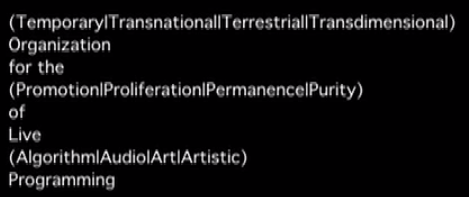
\includegraphics[scale=0.5]{imagens/TOPLAP.png}
  \caption{Definição do siginificado de TOPLAP. \textbf{Fonte}: \citeonline{ramsay_algorithms_2010}.}
  \label{fig:TOPLAP}
\end{figure}

O símbolo ``|'' é uma representação gráfica do operador lógico \emph{OR} (OU), bastante utilizado em algoritmos condicionais. Isto é, \emph{Temporary }| \emph{Trasnational} | \emph{Terrestrial} | \emph{Transdimensional} significa que as letras ímpares ``T'', e ``Ps'', podem significar um ou outro termo indicado pelo algoritmo.

Este comportamento, de permutar ordem das letras é praticado por Nick Collins (1975-); a permutação de suas letras é utilizada pelo pesquisador para gerar pseudônimos como Click Nilson, ou Sick Lincoln. Junto com McLean, Collins cunhou o termo \emph{Algorave}.

\subsection{\emph{Show us your screens}}\label{sec:showusyourscreens}

Além das performances inaugurais nos festivais Europeus, o manifesto Lubeck04, \traducao{iniciado em um ônibus de trânsito Ryanair\disponivelem{https://www.ryanair.com/pt/pt/}, em  Hamburgo, para o aeroporto Lübeck\cite[p.~247]{ward_live_2004}}{begun on a Ryanair transit bus from Hamburg to Lubeck airport}, mais conhecido como ``\emph{Show us your screens}'', prescreve algumas regras práticas do \emph{live coding}. 

\begin{citacao}
Exigimos:

• Acesso à mente do intérprete, para todo o instrumento humano.

• Obscurantismo é perigoso. Mostre-nos suas telas.

• Programas são instrumentos que podem modificar eles mesmos.

• O programa será transcendido - Língua Artificial é o caminho.

• O código deve ser visto assim como ouvido, códigos subjacentes visualizados bem como seu resultado visual.

• Codificação ao vivo não é sobre ferramentas. Algoritmos são pensamentos. Motosserras são ferramentas. É por isso que às vezes algoritmos são mais difíceis de perceber do que motosserras.

Reconhecemos contínuos de interação e profundidade, mas preferimos:

• Introspecção dos algoritmos.

• A externalização hábil de algoritmo como exibição expressiva/impressiva de destreza mental.

• Sem \emph{backup} (minidisc, DVD, safety net computer).

Nós reconhecemos que:

• Não é necessário para uma audiência leiga compreender o código para apreciar, tal como não é necessário saber como tocar guitarra para apreciar uma performance de guitarra.

• Codificação ao vivo pode ser acompanhada por uma impressionante exibição de destreza manual e a glorificação da interface de digitação.

• Performance envolve contínuos de interação, cobrindo talvez o âmbito dos controles, no que diz respeito ao parâmetro espaço da obra de arte, ou conteúdo gestual, particularmente direcionado para o detalhe expressivo. Enquanto desvios na tradicional taxa de reflexos táteis da expressividade, na música instrumental, não são aproximadas no código, por que repetir o passado? Sem dúvida, a escrita de código e expressão do pensamento irá desenvolver suas próprias nuances e costumes. 
\footnote{\loccit{ward_live_2004}. Tradução nossa de:\emph{We demand: \begin{inparaenum}[•]
\item Give us access to the performer's mind, to the whole human instrument.
\item Obscurantism is dangerous. Show us your screens.
\item Programs are instruments that can change themselves.
\item The program is to be transcended - Artificial language is the way.
\item Code should be seen as well as heard, underlying algorithms viewed as well as their visual outcome.
\item Live coding is not about tools. Algorithms are thoughts. Chainsaws are tools. That's why algorithms are
sometimes harder to notice than chainsaws.
\end{inparaenum}. We recognise continuums of interaction and profundity, but prefer:  \begin{inparaenum}[•]
\item Insight into algorithms
\item The skillful extemporisation of algorithm as an expressive/impressive display of mental dexterity
\item No backup (minidisc, DVD, safety net computer)
\end{inparaenum}. We acknowledge that: \begin{inparaenum}[•]
\item It is not necessary for a lay audience to understand the code to appreciate it, much as it is not necessary
to know how to play guitar in order to appreciate watching a guitar performance.
\item Live coding may be accompanied by an impressive display of manual dexterity and the glorification of the
typing interface.
\item Performance involves continuums of interaction, covering perhaps the scope of controls with respect to
the parameter space of the artwork, or gestural content, particularly directness of expressive detail. Whilst
the traditional haptic rate timing deviations of expressivity in instrumental music are not approximated in
code, why repeat the past? No doubt the writing of code and expression of thought will develop its own
nuances and customs.
\end{inparaenum}}}
\end{citacao}

Surgiu como uma resposta ao artigo ``Using Contemporary Technology in Live Performance; the Dilemma of the Performer'' de \citeonline{schloss_dilemma_2003}. A crítica principal de \citeauthoronline{ward_live_2004} refere-se ao sétimo dos questionamentos sugeridos para uma performance de improvisação ao vivo com computadores.

Poderia ser dito que o \emph{live coding} é parte de uma construção histórica de uma tradição musical da \emph{Computer Music Journal}. Porém o documento publicado por \citeauthoronline{ward_live_2004} foi essencial para a divulgação de uma ideologia e de suas regras práticas. Foi escrito como resposta para um problema colocado por \citeonline[p.~241]{schloss_dilemma_2003}:

\begin{citacao}
\traducao{Para reiterar, agora que nós temos computadores rápidos o suficiente para execução ao vivo, nós temos novas possibilidades, e um novo problema. Do começo da evidência arqueológica da música até agora, música era tocada acusticamente, e sempre foi fisicamente evidente como o som era produzido; alí existia uma relação de proximiidade entre gesto e resultado. Agora nós não temos mais que seguir as leis da física (ultimamente temos, mas não nos termos do que o observador vê), uma vez que nós temos completo poder do computador como intérprete e intermediário entre nosso corpo físico e o som produzido. Por esta causa, a ligação entre gesto e resultado foi completamente perdido, se é que existe ligação. Isto significa que nós podemos ir além da relação de causa-e-efeito entre executante e instrumento que faz a mágica. Mágica é bom; muita mágica é fatal }{
To reiterate, now that we have fast enough computers toperform live, we have new possibilities, and a new problem.From the beginning of the archeological evidence of musicuntil now, music was played acoustically, and thus it wasalways physically evident how the sound was produced; there was a nearly one-to-one relationship between gesture andresult. Now we don’t have to follow the laws of physicsanymore (ultimately we do, but not in terms of what theobserver observes), because we have the full power of computers as interpreter and intermediary between our physicalbody and the sound production. Because of this, the link between gesture and result can be completely lost, if indeed there is a link at all. This means that we can go so far beyond the usual cause-and-effect relationship between performer and instrument that it seems like magic. Magic is great; too much magic is fatal
} 
\end{citacao}

Segundo \citeonline[p.~239]{schloss_dilemma_2003}, é necessário: \traducao{considerar a visão do observador sobre os modos de performance das interações físicas e mapeamentos de gestos em som, para fazer uma performance convincente e efetiva}{Its now necessary, (\ldots) ;to consider the observer’s view of the performer’s modes of physical interactions and mappings from gesture to sound, in order to make the performance convincing and effective.}:

\begin{citacao}
\traducao{1. Causa-e-efeito é importante, pelo menos para o observador/audiência em uma sala de concerto. 
\ \\
2.Corolário: Mágica na performance é bom. Muita mágica é fatal! (chato).
\ \\
3. Um componente visual é essencial para a audiência, tal como existe um aparato visual de entrada para parâmetros e gesos.
\ \\
4. Sutileza é importante. Grandes gestos são facilmente visíveis de longe, o que é bom, mas eles são movimentos de desenho animado se comparados à execução de um instrumento musical.
\ \\
5. Esforço é importante. Neste sentido, nós estamos em desvantagem de desempenho na performance musical com o computador.
\ \\
6. Improvisação no palco é bom, mas ``mimar'' o aparato no palco não é improvisação, é edição. É provavelmente mais apropriado fazer isso no estúdio antes do concerto, ou se durante o concerto, com o console no meio ou atrás da sala de concerto.
\ \\
7. Pessoas que representam devem representar. Um concerto de música de computador não é uma desculpa/oportunidade para um programador(a) se sentar no palco. Sua presença melhora ou impede o desempenho da representação?
}{1. Cause-and-effect is important, at least for the observer/audience in a live concert venue. 2. Corollary: Magic in a performance is good. Too much magic is fatal! (Boring). 3. A visual component is essential to the audience, such that there is a visual display of input parameters/gestures. The gestural aspect of the sound becomes easier to experience. 4. Subtlety is important. Huge gestures are easily visible from far away, which is nice, but they are cartoon- movements compared to playi
ng a musical instrument. 5. Effort is important. In this regard, we are handicapped in computer music performance. 6. Improvisation on stage is good, but “baby-sitting” the apparatus on stage is not improvisation, it is editing. It is probably more appropriate to do this either in the studio before the concert, or if at the concert, then at the console in the middle or back of the concert hall. 7. People who perform should be performers. A computer music concert is not an excuse/opportunity for a computer programmer to finally be on stage. Does his/her presence enhance the performance or hinder it?} \end{citacao}

Escolhemos um ponto de interesse particular; a frase ``Algoritmos são pensamentos, motosserras são ferramentas'' foi muito discutida no processo de qualificação desta tese. Particularmente, existe um vídeo , em formato de \emph{Vlog}, que discute o \emph{live coding} sob esta perspectiva.
 
\subsubsection{Algorithms are Thoughts, Chainsaws are Tools}

``Algorithms are Thoughts, Chainsaws are Tools'' é o nome dado ao vídeo de Stephen \citeonline{ramsay_algorithms_2010}, publicado no Vimeo, em  27 de fevereiro de 2010, como um \emph{Coffee-Table Movie}. É uma análise pessoal da performance de \emph{Strange Places} de Andrew Sorensen. O nome do vídeo é derivado de uma das regras práticas apresentadas na \autoref{sec:showusyourscreens}, p. \pageref{sec:showusyourscreens}; mais especificamente, o sexto item:

\begin{citacao}
Codificação ao vivo não é sobre ferramentas. Algoritmos são pensamentos. Motosserras são ferramentas. É por isso que às vezes algoritmos são mais difíceis de perceber do que motosserras \cite[p.~22; item 6]{griffiths_fluxus:_2008}.
\end{citacao}

O algoritmo como pensamento é um Espaço Conceitual abstrato; pode conter qualquer fundamento teórico pertinente para uma improvisação específica. O dispositivo usado (motoserra, máquina de tecelagem ou o computador) é um meio pelo qual o algoritmo toma sua forma sonora. É interessante aqui notar que este vídeo contém uma descrição e comentários que podem elucidar a frase-alvo sob o prisma da partitura musical. Abaixo realizei uma compilação de fragmentos de alguns dos comentários que considerei pertinentes. Ramsey apresenta a seguinte descrição do vídeo:

\begin{citacao}
Um curta sobre \emph{livecoding} apresentado como parte do Grupo de Estudos de Crítica de Códigos, em 2010, por Stephen Ramsay. Apresenta uma leitura ao vivo $[$\emph{live reading}$]$ de uma performance do compositor Andrew Sorensen. Também fala sobre J.D. Salinger, the Rockets, tocando instrumentos, Lisp, do clima em Brisbane e tímpanos \footnote{\loccit{ramsay_algorithms_2010} Tradução de \emph{A short film on livecoding presented as part of the Critical Code Studies Working Group, March 2010, by Stephen Ramsay. Presents a "live reading" of a performance by composer Andrew Sorensen. It also talks about J. D. Salinger, the Rockettes, playing musical instruments, Lisp, the weather in Brisbane, and kettle drums.}.}.
\end{citacao}

Amanda French nega a utilização do termo \emph{partitura} para explicitar diferenças no uso da programação-partitura, em uma performance de improvisação com o computador, para uma performance não-improvisada com partitura.

\begin{citacao}
A noção de partitura não se aplica aqui, é como não fosse possível aplicá-lo ao músico de \emph{jazz} ou tocador de \emph{bluegrass}. (\ldots). Levanta a questão, para mim, se, em uma sessão de \emph{livecoding} *feita*, constite simplismente no ato de digitar em um programa existente, seria tão convincente -- Eu acho que isso pode definitivamente ter pontos de interesse. Ou qual seria o análogo do \emph{livecoding} para uma performance não-improvisada de música?\footnote{\loccit{ramsay_algorithms_2010} Tradução parcial de \emph{The notion of "sheet music" doesn't apply here, as it wouldn't apply to a jazz musician or a bluegrass picker. Even the name of his environment, Impromptu, makes that point. Raises the question for me precisely of whether a livecoding session that *did* consist of simply typing in an existing program would be as compelling -- I think it would definitely have its points of interest, actually. Or what would the livecoding analog be to a non-improvisational live performance of music?}}
\end{citacao}

Um segundo comentário de Matt King, coloca a pergunta de Amanda em outra perspectiva:

\begin{citacao}
O que torna o \emph{livecoding} diferente, e pode a performance de música tradicional imitar isso? Para responder esta questão, parece importante notar que as formas nas quais a música improvisada muitas vezes apela para alguma noção de autenticidade ou gênio. Enquanto o \emph{livecoding} ele mesmo à noção de virtuosismo de código, ``autenticidade'' parece fora de lugar aqui. Se música improvisada sugere expressão, o \emph{livecoding} sugere um conjunto de restrições na expressão, descrevendo os parâmetros através dos quais a máquina $[$midi$]$ ganha expressão \footnote{Tradução nossa de \emph{(\ldots) What makes livecoding different, and can a traditional music performance mimic it? To answer this question, it seems important to note the ways in which improvised music often appeals to some notion of authenticity or genius. While livecoding might lend itself to some notion of coding virtuosity, "authenticity" seems out of place here. If improvised music is expression, livecoding suggests a setting of constraints on expression, describing the parameters through which the machine (midi) gets expressed.}}
\end{citacao}

Michel Pasin defende que o ato de improvisação musical requer conhecimentos técnicos prévios, mas não necessariamente correlacionados ao conhecimento do que é uma partitura: \traducao{Em geral, é somente dominando um instrumento que você pode esquecer sobre a técnica e concentrar em 'dizer' coisas com o instrumento.}{In general, it is only by mastering an instrument that you can forget about the technique and concentrate on 'saying' things with the instrument.}. 

\subsubsection{Obscurantismo é perigoso, mostre-nos suas telas}\label{sec:obscurantismo}